\chapter{El átomo de hidrógeno}\label{ch:b3:hydrogen-atom}

Nueve de cada diez átomos del universo son hidrógeno: un protón que retiene
un electrón, el único átomo que la física resuelve exactamente --- y la
llave que abrió todos los demás. La vieja teoría cuántica del
\cref{ch:b3:hamiltonian-mechanics} adivinó sus energías; la maquinaria está
ya dispuesta para \emph{deducirlas}: el potencial de Coulomb entra en la
\omterm{prop:b3:schrodinger-three-dimensions:swave}{ecuación radial} del capítulo anterior y de ella salen los niveles
$-E_{\text{I}}/n^2$, el \omterm{thm:b3:hydrogen-atom:levels}{radio de Bohr}, las capas y subcapas de la tabla
periódica de la química y las series espectrales que los astrónomos leen en
cualquier nebulosa. La misma solución, reescalada, describe el helio
ionizado, los átomos muónicos, el positronio y los ``átomos'' de
electrón--hueco del interior de los semiconductores; estirada hasta $n
\approx 100$ describe átomos de Rydberg de medio micrómetro de anchura,
cuyos susurros de radio cartografían las nubes ionizadas de la Galaxia y
cuyas interacciones gobiernan hoy ordenadores cuánticos.
% NOTE: full radial solutions (Laguerre) admitted; ground state solved
% exactly; emphasis on scaling laws and applications.

\section{El problema de Coulomb, resuelto}

\begin{theorem}[Niveles del hidrógeno]\label{thm:b3:hydrogen-atom:levels}
\index{átomo de hidrógeno}\index{número cuántico principal}\index{radio de Bohr}
Para $V(r) = -e^2/4\pi\varepsilon_0 r$ (escribiendo $k = e^2/4\pi
\varepsilon_0$), los estados ligados se etiquetan $(n, l, m)$ con
\[
E_n = -\frac{E_{\text{I}}}{n^2} , \qquad
E_{\text{I}} = \frac{m_{\text{e}}k^2}{2\hbar^2} = \qty{13.6}{eV} ,
\qquad n = 1, 2, 3, \dots
\]
y, para cada $n$, los números orbitales $l = 0, 1, \dots, n-1$ y
$m = -l, \dots, l$. La longitud natural es el \omterm{thm:b3:hydrogen-atom:levels}{radio de Bohr} $a_0 =
\hbar^2/m_{\text{e}}k = \qty{52.9}{pm}$; el estado fundamental es
\[
\psi_{100} = \frac{1}{\sqrt{\pi a_0^3}}\;\eu^{-r/a_0} .
\]
La energía depende \emph{solo} de $n$: contando las $m$ y las
$l$, el nivel $n$ tiene degeneración $n^2$ (duplicada por el espín,
\cref{ch:b3:spin-two-level}) --- mucho más allá de la degeneración
$(2l+1)$ que explica la isotropía.
\end{theorem}

\begin{proof}[Demostración parcial]
Para el estado fundamental, pruébese $u = Cr\,\eu^{-r/a}$ en la \omterm{prop:b3:schrodinger-three-dimensions:swave}{ecuación
radial} con $l = 0$: $u'' = (1/a^2 - 2/ar)u$, de modo que
$-\tfrac{\hbar^2}{2m_{\text{e}}}u'' - \tfrac kr u = Eu$ exige
$\hbar^2/m_{\text{e}}a = k$ (igualando los términos en $1/r$) --- es decir,
$a = a_0$ --- y $E = -\hbar^2/2m_{\text{e}}a_0^2 = -E_{\text{I}}$.
La solución general (polinomios de Laguerre, con $n - l - 1$ nodos
radiales) se admite; cada paso de la construcción es elemental, pero
largo. La degeneración ``accidental'' en $l$ refleja un secreto clásico
de la fuerza $1/r$ pura --- las elipses de Kepler no precesan, y un
vector conservado adicional (el de Laplace--Runge--Lenz) apunta a lo largo
del eje mayor fijo; su versión cuántica es lo que ata distintos $l$ a una
sola energía (\cref{exo:b3:hydrogen-atom:12}).
\end{proof}

\begin{omfigure}
\begin{tikzpicture}[font=\small, >=Stealth]
  % energy scale: E = -13.6/n^2, map E -> y = 5.6 + E*0.42 (E in eV)
  % n=1: y=-0.11? choose y(E) = 5.9 + 0.42*E: n1: 0.19, n2: 4.47, n3: 5.27, n4: 5.55, inf: 5.9
  \draw[->] (-0.4,-0.4) -- (-0.4,6.6);
  \node[anchor=south] at (-0.4,6.6) {$E$ (eV)};
  % continuum
  \fill[gray!15] (0,5.9) rectangle (8.6,6.45);
  \node[anchor=west, font=\footnotesize] at (8.7,6.15) {continuo: ionizado};
  \draw[thick] (0,5.9) -- (8.6,5.9);
  \node[anchor=east, font=\footnotesize] at (-0.5,5.9) {$0$};
  % levels, split by l columns
  \foreach \n/\y in {1/0.19, 2/4.47, 3/5.27, 4/5.55}
    {\node[anchor=east, font=\footnotesize] at (-0.5,\y) {$-13.6/\n^2$};}
  % l columns: s at x 0-1.4, p at 1.9-3.3, d at 3.8-5.2, f 5.7-7.1
  \node[font=\footnotesize] at (0.7,-0.3) {$l = 0$ ($s$)};
  \node[font=\footnotesize] at (2.6,-0.3) {$l = 1$ ($p$)};
  \node[font=\footnotesize] at (4.5,-0.3) {$l = 2$ ($d$)};
  \node[font=\footnotesize] at (6.4,-0.3) {$l = 3$ ($f$)};
  \draw[very thick, omDef] (0,0.19) -- (1.4,0.19);
  \foreach \x in {0,1.9} \draw[very thick, omDef] (\x,4.47) -- ({\x+1.4},4.47);
  \foreach \x in {0,1.9,3.8} \draw[very thick, omDef] (\x,5.27) -- ({\x+1.4},5.27);
  \foreach \x in {0,1.9,3.8,5.7} \draw[very thick, omDef] (\x,5.55) -- ({\x+1.4},5.55);
  % series arrows
  \draw[->, omExo, thick] (0.5,4.47) -- (0.6,0.24);
  \draw[->, omExo, thick] (1.0,5.27) -- (0.85,0.24);
  \node[omExo, font=\footnotesize, anchor=west] at (0.95,2.3) {Lyman (UV)};
  \draw[->, omThm, thick] (2.6,5.27) -- (2.45,4.52);
  \draw[->, omThm, thick] (3.1,5.55) -- (2.9,4.52);
  \node[omThm, font=\footnotesize, anchor=west] at (3.25,4.95) {Balmer (visible)};
  \node at (1.9,1.55) {};
\end{tikzpicture}

{\small Los niveles del hidrógeno $-E_{\text{I}}/n^2$, desplegados según
$l$: todas las subcapas de un mismo $n$ coinciden (el ``accidente'' de
Coulomb). Los saltos hacia abajo que terminan en $n = 1$ forman la serie
ultravioleta de Lyman; los que terminan en $n = 2$, la serie visible de
Balmer que tiñe de rojo las nebulosas.}
\end{omfigure}

\section{Dónde está el electrón}

\begin{proposition}[Distribuciones radiales]\label{prop:b3:hydrogen-atom:radial}
\index{probabilidad radial}
La probabilidad de hallar el electrón entre $r$ y $r + \dd r$
es $P(r)\,\dd r$ con $P(r) = |u(r)|^2$, el cuadrado de la
función radial normalizada del \cref{thm:b3:quantum-angular-momentum:radial}. Para los estados más bajos:
$P_{1s} \propto r^2\eu^{-2r/a_0}$, con máximo exactamente en $r = a_0$ y
$\langle r\rangle = \tfrac32 a_0$; $P_{2s}$ muestra dos jorobas
separadas por un \emph{nodo} esférico; $P_{2p} \propto
r^4\eu^{-r/a_0}$, con máximo en $4a_0$. En general, $\langle r\rangle
\approx n^2a_0$: los átomos crecen \emph{cuadráticamente} con la
excitación, mientras que su energía de enlace se encoge como $1/n^2$ --- la palanca
que hay tras los gigantes de Rydberg del \cref{pb:b3:hydrogen-atom:1}.
\end{proposition}
\admitted

\begin{omfigure}
\begin{tikzpicture}
  \begin{axis}[omaxis, axis x line=bottom, axis y line=left,
    width=11.6cm, height=5.8cm, xmin=0, xmax=14, ymin=0, ymax=0.62,
    xlabel={$r/a_0$}, ylabel={$P(r)$ (por $a_0$)},
    xlabel style={at={(axis description cs:0.5,-0.1)}, anchor=north},
    xtick={1,4,5,10}, ytick=\empty, clip=false,
    legend style={font=\scriptsize, at={(0.95,0.9)}, anchor=north east,
      draw=none, fill=none}]
    \addplot[omDef, very thick, domain=0:8, samples=120] {4*x*x*exp(-2*x)};
    \addlegendentry{$1s$}
    \addplot[omThm, thick, domain=0:14, samples=140] {0.125*x*x*(2-x)^2*exp(-x)};
    \addlegendentry{$2s$}
    \addplot[omExo, thick, domain=0:14, samples=140] {x^4*exp(-x)/24};
    \addlegendentry{$2p$}
    \draw[gray, dashed] (axis cs:1,0) -- (axis cs:1,0.545);
  \end{axis}
\end{tikzpicture}

{\small Densidades de \omterm{prop:b3:hydrogen-atom:radial}{probabilidad radial}. El máximo del $1s$ se sitúa
exactamente en $a_0$; el estado $2s$ lleva un nodo esférico y un lóbulo
cerca del núcleo --- la ``penetración'' que ordenará la tabla periódica
---, mientras que el $2p$, amurallado por la \omterm{thm:b3:quantum-angular-momentum:radial}{barrera centrífuga}, se
mantiene apartado.}
\end{omfigure}

\begin{example}[Leer los tamaños]\label{ex:b3:hydrogen-atom:sizes}
Estado fundamental: \qty{0.1}{nm} de anchura y \qty{13.6}{eV} de
profundidad --- las escalas de toda la química. En $n = 10$: radio
$\sim\qty{5}{nm}$ y energía de enlace de \qty{0.136}{eV} --- retenido con
flojedad. En $n = 100$: un átomo de escala \emph{micrométrica} ligado por
\qty{1.4}{meV}, destrozado por el campo más endeble --- y, sin embargo, el
espacio interestelar está lo bastante vacío para que tales átomos vivan y
emitan (\cref{pb:b3:hydrogen-atom:1}).
\end{example}

\section{El espectro}

\begin{proposition}[Series y reglas de selección]\label{prop:b3:hydrogen-atom:series}
\index{serie de Balmer}\index{serie de Lyman}
Un salto $n' \to n$ emite la longitud de onda
\[
\frac{1}{\lambda} = R_{\text{H}}\Big(\frac{1}{n^2} -
\frac{1}{n'^2}\Big) , \qquad
R_{\text{H}} = \frac{E_{\text{I}}}{hc} = \qty{1.097e7}{m^{-1}} ,
\]
sujeta a la regla de selección dipolar $\Delta l = \pm1$ (el fotón
lleva $\hbar$). La \omterm{prop:b3:hydrogen-atom:series}{serie de Lyman} ($\to n = 1$) cae en el ultravioleta
lejano a partir de \qty{121.6}{nm}; la \omterm{prop:b3:hydrogen-atom:series}{serie de Balmer} ($\to n = 2$)
empieza en la línea roja $H\alpha$, de \qty{656.3}{nm} --- el color de las
nebulosas de emisión y de las protuberancias solares ---; las series de
Paschen y posteriores se retiran al infrarrojo, y entre $n = 110$ y $109$
la misma fórmula aterriza en \qty{5.0}{GHz}: el hidrógeno habla desde el
ultravioleta hasta el dial de radio.
\end{proposition}

\begin{proof}
Conservación de la energía con el \cref{thm:b3:hydrogen-atom:levels};
$R_{\text{H}}$ como en el \cref{pb:b3:hamiltonian-mechanics:1}, ahora
deducido en lugar de postulado.
\end{proof}

\begin{example}[Átomos hidrogenoides: una solución, muchos átomos]\label{ex:b3:hydrogen-atom:scaling}
Sustitúyase la carga del protón por $Ze$ y el electrón por cualquier masa
$\mu$ en órbita: toda fórmula se reescala como
\[
a \to a_0\,\frac{m_{\text{e}}}{\mu}\,\frac1Z , \qquad
E_{\text{I}} \to E_{\text{I}}\,\frac{\mu}{m_{\text{e}}}\,Z^2 .
\]
He$^+$ ($Z = 2$): \qty{54.4}{eV}. Electrones internos de los átomos pesados
($Z \sim 30$): energías de la capa K en el keV --- los rayos X
característicos con los que Moseley ordenó los elementos
(\cref{exo:b3:hydrogen-atom:5}). Hidrógeno muónico ($\mu = 207
m_{\text{e}}$): un átomo de escala femtométrica que sondea el protón mismo.
Positronio ($e^+e^-$, $\mu = m_{\text{e}}/2$): la mitad de energía de enlace,
el doble de tamaño y una vida breve que acaba en fotones de aniquilación.
Y en un semiconductor, un electrón y un hueco se orbitan mutuamente
con masas efectivas pequeñas dentro de un dieléctrico que apantalla: un
\emph{excitón}, el mismo átomo crecido hasta los diez nanómetros y los
milielectronvoltios (\cref{exo:b3:hydrogen-atom:7}) --- el hidrógeno es
menos un átomo que una plantilla.
\end{example}

\begin{omfigure}
\begin{tikzpicture}[font=\small]
  % size comparison, hand-drawn
  \draw[omDef, thick, fill=omDef!12] (1.2,0) circle (1.05);
  \fill[omDef] (1.2,0) circle (1.5pt);
  \node[align=center, font=\footnotesize] at (1.2,-1.75)
    {hidrógeno\\$a_0$, \qty{-13.6}{eV}};
  \draw[omThm, thick, fill=omThm!12] (4.6,0) circle (0.42);
  \fill[omThm] (4.6,0) circle (1.5pt);
  \node[align=center, font=\footnotesize] at (4.6,-1.75)
    {H muónico\\$a_0/207$ (aquí $\times 40$)\\\qty{-2.5}{keV}};
  \draw[omExo, thick, fill=omExo!12] (8.1,0) circle (1.55);
  \fill[omExo] (8.1,0) circle (1.5pt);
  \node[align=center, font=\footnotesize] at (8.1,-2.25)
    {positronio\\$2a_0$, \qty{-6.8}{eV}};
  \draw[omProp, thick, fill=omProp!10] (12.4,0) circle (2.0);
  \fill[omProp] (12.4,0) circle (1.5pt);
  \node[align=center, font=\footnotesize] at (12.4,-2.75)
    {excitón en un cristal\\$\sim 170\,a_0$ (aquí $\div 50$)\\$\sim\qty{-7}{meV}$};
\end{tikzpicture}

{\small Una solución, cuatro ``átomos'': reescalar la masa, la carga y el
entorno dieléctrico convierte al hidrógeno en sondas del protón, pruebas de
electrodinámica cuántica pura y los cuasiátomos emisores de luz de los
semiconductores.}
\end{omfigure}

\begin{method}[Trabajar con sistemas hidrogenoides]\label{met:b3:hydrogen-atom:method}
(1) Escalar primero: $a \propto 1/\mu Z$ y $E \propto \mu Z^2$ convierten
cualquier respuesta del hidrógeno en la de cualquier hidrogenoide.
(2) Tamaños: $\langle
r\rangle \sim n^2a$; espaciados cerca del nivel $n$: $\dd E/\dd n =
2E_{\text{I}}/n^3$. (3) Espectros: fórmula de Rydberg más $\Delta l =
\pm1$. (4) Penetración: los estados $s$ sienten el núcleo y los
de $l$ alto orbitan por fuera --- la palanca de la química de muchos
electrones. (5) Anclas de sensatez: $\qty{13.6}{eV}$, $\qty{52.9}{pm}$,
$\qty{121.6}{nm}$ y $\qty{656.3}{nm}$ --- cuatro números que merece la pena
memorizar de por vida.
\end{method}

\begin{omfigure}
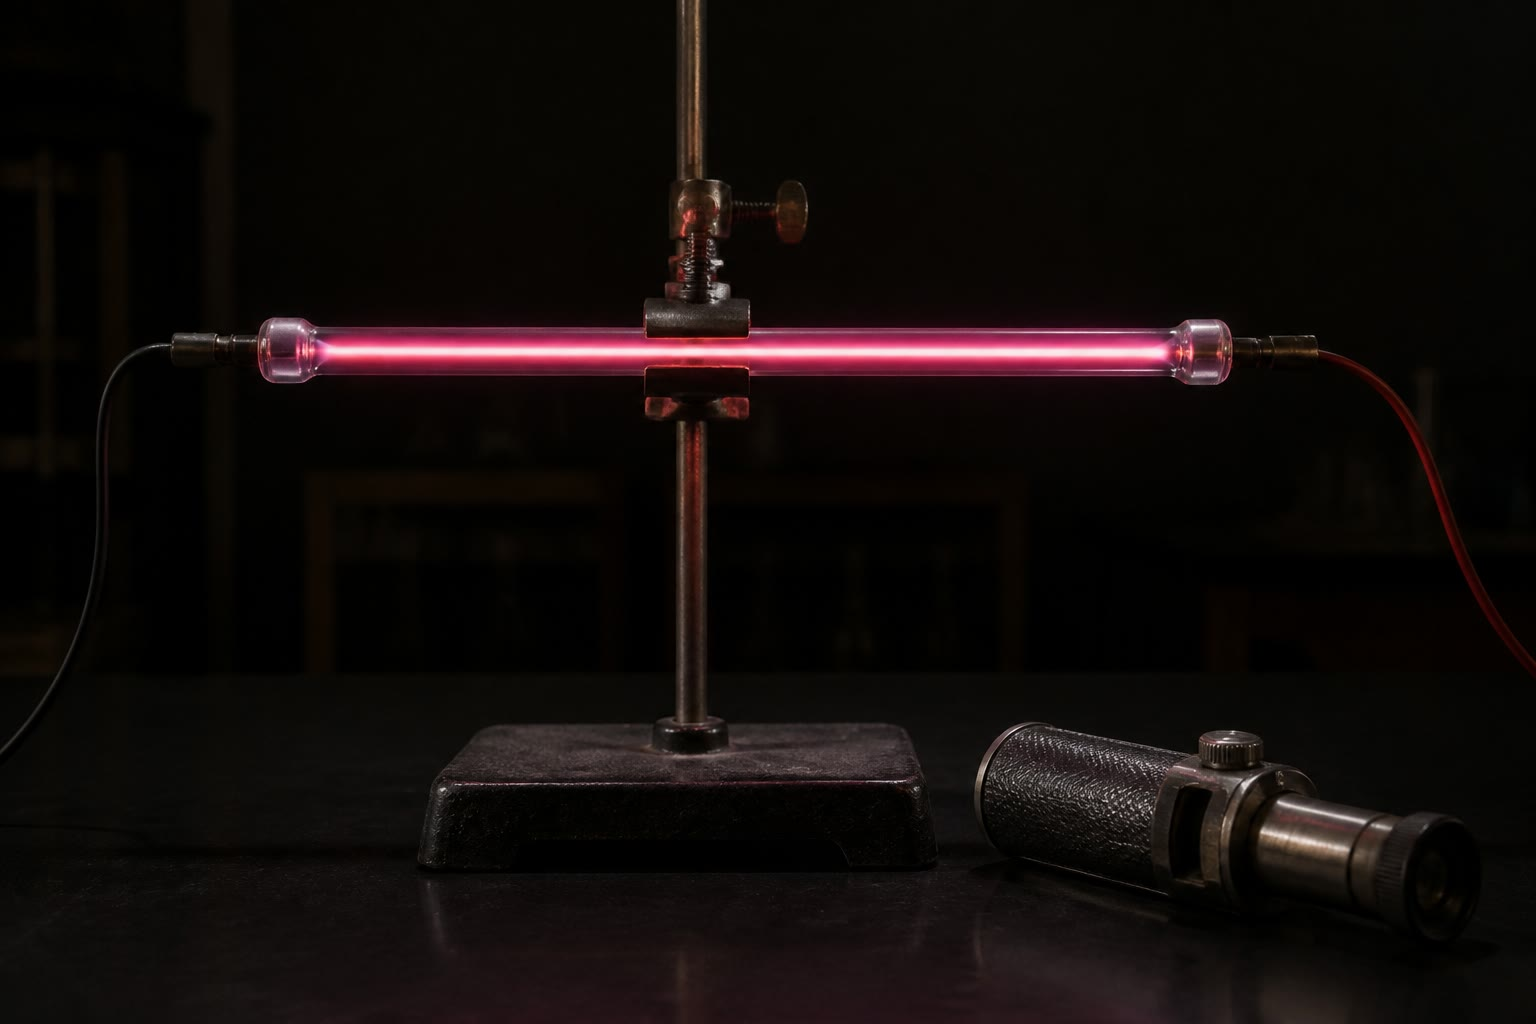
\includegraphics[width=0.58\linewidth]{images/book5/ai/b5-11-discharge-tube.jpg}

{\small Un tubo de descarga de hidrógeno y un espectroscopio de bolsillo: el resplandor rosado, descompuesto, se convierte en las líneas de Balmer --- la huella entera que este capítulo deduce del potencial de Coulomb.}
\end{omfigure}

\section{Ejercicios}

\begin{exercise}[$\star$]\label{exo:b3:hydrogen-atom:1}
(a) Verifíquese por sustitución que $u = Cr\eu^{-r/a_0}$ resuelve la
\omterm{prop:b3:schrodinger-three-dimensions:swave}{ecuación radial} con $l = 0$ y $E = -E_{\text{I}}$, siempre que $a_0 =
\hbar^2/m_{\text{e}}k$. (b) Normalícese ($\int_0^\infty
x^2\eu^{-x}\dd x = 2$). (c) Compruébense las dimensiones de $a_0$ y de
$E_{\text{I}}$. (d) ¿Por qué no hay ningún estado por debajo de
$-E_{\text{I}}$ (arguméntese con el
\cref{exo:b3:schrodinger-three-dimensions:12})?
\end{exercise}

\begin{exercise}[$\star$]\label{exo:b3:hydrogen-atom:2}
Calcúlense (a) las longitudes de onda de Lyman $\alpha$ y del límite de
Lyman; (b) las tres primeras líneas de Balmer y el límite de Balmer ---
¿cuáles son visibles y de qué colores?; (c) el rango de la serie de Paschen;
(d) la frecuencia de la transición $n = 110 \to 109$.
\end{exercise}

\begin{exercise}[$\star$]\label{exo:b3:hydrogen-atom:3}
Para el estado fundamental: (a) localícese el máximo de $P_{1s}(r)$; (b)
calcúlese $\langle r\rangle$; (c) calcúlese la probabilidad de hallar el
electrón más allá de $2a_0$ ($\int_x^\infty t^2\eu^{-t}\dd t = (x^2 +
2x + 2)\eu^{-x}$); (d) ¿por qué inducen a error las imágenes de una
``órbita'' de radio exactamente $a_0$?
\end{exercise}

\begin{exercise}[$\star$]\label{exo:b3:hydrogen-atom:4}
(a) Enumérense las parejas $(l, m)$ de $n = 3$ y verifíquese el recuento $n^2 =
9$. (b) Con el espín, ¿cuántos estados hay en las capas $n = 1, 2, 3$? (c)
Hágase corresponder esos números con las longitudes $2, 8, 18$ de las filas de
la tabla periódica. (d) ¿Qué degeneración (en $m$ o en $l$) sobrevive en el
electrón externo del sodio, y por qué se rompe la otra?
\end{exercise}

\begin{exercise}[$\star\star$]\label{exo:b3:hydrogen-atom:5}
La escalera de Moseley. Un electrón interno (de la capa K) de un elemento
$Z$ se mueve en un campo nuclear casi desnudo, apantallado por el otro
electrón K: carga efectiva $\approx Z - 1$. (a) Muéstrese que la energía
del rayo X $2p \to 1s$ vale aproximadamente $\tfrac34(Z-1)^2E_{\text{I}}$.
(b) Evalúese para el cobre ($Z = 29$) y compárese con la K$\alpha$ medida en
\qty{8.05}{keV}. (c) Moseley (1913) representó
$\sqrt{\nu}$ frente a $Z$ y obtuvo rectas: ¿qué demostró eso sobre el
significado del número atómico? (d) Predígase la energía K$\alpha$
del entonces ausente elemento $Z = 43$.
\end{exercise}

\begin{exercise}[$\star\star$]\label{exo:b3:hydrogen-atom:6}
Positronio. (a) Justifíquese $\mu = m_{\text{e}}/2$ y dense su energía de
energía de enlace y su \omterm{thm:b3:hydrogen-atom:levels}{radio de Bohr}. (b) Su longitud de onda Lyman $\alpha$.
(c) El parapositronio se aniquila en dos fotones: sus energías
y sus direcciones relativas (a partir del \cref{ch:b3:relativistic-dynamics}).
(d) ¿Dónde detecta la medicina exactamente esta firma a diario?
\end{exercise}

\begin{exercise}[$\star\star$]\label{exo:b3:hydrogen-atom:7}
Excitones. En el arseniuro de galio, $\varepsilon_{\text{r}} = 12.9$ y
la masa efectiva reducida es $\mu = 0.058\,m_{\text{e}}$. (a) Muéstrese que
$a_{\text{ex}} = a_0\,\varepsilon_{\text{r}}\,m_{\text{e}}/\mu$ y
evalúese. (b) La energía de enlace del excitón. (c) Compárese
$a_{\text{ex}}$ con los radios de punto cuántico del
\cref{pb:b3:schrodinger-three-dimensions:1} y justifíquese, por fin,
despreciar el término de Coulomb en los puntos pequeños. (d) ¿Por qué
aparecen las líneas excitónicas solo en semiconductores \emph{puros y
fríos} ($k_{\text{B}}T$ frente a su respuesta al apartado (b))?
\end{exercise}

\begin{exercise}[$\star\star$]\label{exo:b3:hydrogen-atom:8}
Penetración y los metales alcalinos. El sodio es un electrón de valencia
hidrogenoide fuera de un tronco cerrado de carga efectiva $+e$.
(a) ¿Cuál de los estados $3s$, $3p$ o $3d$ siente más el núcleo
incompletamente apantallado, y por qué (recuérdese la figura radial)? (b) Los
niveles medidos son $E_{3s} = \qty{-5.14}{eV}$, $E_{3p} = \qty{-3.04}{eV},
E_{3d} = \qty{-1.52}{eV}$: compruébese que el $3d$ es casi hidrogenoide
($n = 3$) mientras que el $3s$ es mucho más profundo, y explíquese. (c)
Calcúlese la longitud de onda de $3p \to 3s$: ¿qué color célebre es ese? (d)
Escríbanse los niveles alcalinos como $-E_{\text{I}}/(n - \delta_l)^2$ y
extráiganse los ``defectos cuánticos'' $\delta_s$ y $\delta_p$ del sodio.
\end{exercise}

\begin{exercise}[$\star\star$]\label{exo:b3:hydrogen-atom:9}
Un protón de una nebulosa captura un electrón en $n = 100$. (a) ¿Cuánta
energía se libera en el fotón de captura si el electrón llegó casi libre?
(b) El átomo desciende en cascada, preferentemente por pasos con
$\Delta n = 1$ a $n$ alto: ¿en qué banda caen esos fotones? (c) El último
paso de la cascada es Lyman $\alpha$; la luz visible de las nebulosas está
dominada por H$\alpha$: rastréese a qué paso de la cascada corresponde. (d)
Explíquese por qué las nebulosas de emisión brillan en \emph{rojo} aunque la
línea más intensa del hidrógeno (Lyman $\alpha$) sea ultravioleta.
\end{exercise}

\begin{exercise}[$\star\star\star$]\label{exo:b3:hydrogen-atom:10}
Promedios y virial. Para el estado fundamental, calcúlese (a)
$\langle 1/r\rangle$ y compruébese que $\langle E_p\rangle = -2E_{\text{I}}
= 2E_1$; (b) $\langle E_k\rangle = +E_{\text{I}}$, verificando la
razón del virial del \cref{exo:b3:hamiltonian-mechanics:4}; (c) la
velocidad cuadrática media del electrón y $v/c$; (d) el orden de magnitud del campo magnético que
experimenta el \emph{protón} debido al movimiento del electrón (una espira
de corriente $ev/2\pi a_0$ vista a distancia $a_0$) --- un número que la
estructura hiperfina necesitará.
\end{exercise}

\begin{exercise}[$\star\star\star$]\label{exo:b3:hydrogen-atom:11}
Cuán fina es la estructura fina. (a) Muéstrese que la escala de velocidad
del estado fundamental es $\langle v^2\rangle^{1/2}/c = \alpha \approx 1/137$
y, para un hidrogenoide de carga $Z$: $Z\alpha/n$. (b) Las correcciones
relativistas entran en el orden relativo $(v/c)^2$: estímense la escala de la
estructura fina $\alpha^2E_{\text{I}}$ en meV, y el orden del
desdoblamiento para $n = 2$ en GHz. (c) Para el uranio hidrogenoide
($Z = 92$): $v/c$ en $n = 1$ --- ¿es sostenible el tratamiento no
relativista? (d) ¿Qué anuncia físicamente la divergencia formal en
$Z\alpha \to 1$ ($Z \approx 137$)?
\end{exercise}

\begin{exercise}[$\star\star\star$]\label{exo:b3:hydrogen-atom:12}
La degeneración irrazonable. (a) En mecánica clásica, muéstrese que
para $V = -k/r$ la órbita se cierra (sin precesión) citando el
vector conservado de Laplace--Runge--Lenz $\vect A = \vect p\wedge\vect
L - mk\,\vect e_r$ --- verifíquese $\dd\vect A/\dd t = 0$ usando la ley de
Newton. (b) Arguméntese: un vector conservado que fija el eje de la elipse es
una simetría adicional más allá de las rotaciones --- y una simetría
adicional significa degeneración adicional (recuérdese el
\cref{exo:b3:quantum-formalism:9}). (c) Añádase una
pequeña corrección en $1/r^2$ al potencial y muéstrese que la elipse
precesa: el eje gira y $\vect A$ deja de conservarse. (d)
Conéctese: en los átomos multielectrónicos el potencial efectivo no es
$1/r$ puro, y la degeneración en $l$ se rompe (¡el sodio!); en el hidrógeno
mismo, la relatividad suministra la pequeña corrección --- ¿qué rasgo
observado del \cref{exo:b3:hydrogen-atom:11} es ese?
\end{exercise}

\section{Problema: átomos gigantes}

\begin{problem}[{Problema de fin de semana --- átomos de Rydberg, del
resplandor de radio de la Galaxia a los ordenadores cuánticos}]\label{pb:b3:hydrogen-atom:1}
Estírese el hidrógeno hasta $n \approx 100$ y se convertirá en otra clase de
objeto: de micrómetros de anchura, ligado por milielectronvoltios,
absurdamente sensible --- y absurdamente útil. Este problema escala la
solución del hidrógeno hacia arriba, primero hasta las nubes interestelares
que emiten en longitudes de onda centimétricas y luego hasta los arreglos de
laboratorio en los que tales gigantes se entrelazan formando procesadores.
Datos: $E_{\text{I}} = \qty{13.6}{eV}$, $a_0 = \qty{52.9}{pm}$,
$R_{\text{H}}c = \qty{3.29e15}{Hz}$; $k_{\text{B}}T$ a
\qty{300}{K} vale \qty{25.9}{meV}.

\medskip\noindent\textbf{Parte I --- Las leyes de escala.}
\begin{enumerate}
  \item Dense las cuatro dependencias básicas con $n$: el tamaño $\langle
        r\rangle$, la energía de enlace $|E_n|$, el espaciado $E_{n+1} - E_n$ (para
        $n$ grande) y la frecuencia orbital clásica de la
        órbita de Bohr correspondiente.
  \item Muéstrese que, para $n$ grande, la frecuencia de transición $n+1 \to
        n$ tiende a $2R_{\text{H}}c/n^3$, y verifíquese que es
        igual a la frecuencia orbital clásica (el principio de
        correspondencia del \cref{pb:b3:hamiltonian-mechanics:1},
        completado).
  \item Evalúense el tamaño y la energía de enlace en $n = 50$ y en $n = 100$.
  \item El dipolo eléctrico de un átomo de Rydberg va como $n^2ea_0$:
        evalúese en $n = 50$ en debyes ($1\,\text{D} =
        \qty{3.34e-30}{C.m}$) y compárese con los \qty{1.85}{D} de una
        molécula de agua.
  \item Estímese el campo eléctrico que desgarra el átomo con $n = 50$,
        como $F \sim |E_n|/(e\,\langle r\rangle)$, en V/cm.
  \item ¿Por qué no pueden sobrevivir tales átomos a la química ordinaria
        del vacío de laboratorio y sí lo hacen sin problema en el espacio
        interestelar (compárense los ritmos de colisión)?
\end{enumerate}

\medskip\noindent\textbf{Parte II --- Las líneas de recombinación de la
Galaxia.}
En las nebulosas ionizadas, los protones capturan electrones en $n$ altos; la
cascada radia un peine de ``líneas de recombinación de radio''.
\begin{enumerate}[resume]
  \item Calcúlese la frecuencia de la transición $n = 110 \to 109$
        (llamada H109$\alpha$).
  \item ¿En qué banda cae y qué clase de telescopio la recibe?
  \item Calcúlese la longitud de onda de H109$\alpha$ y compárese con
        el tamaño del átomo emisor: ¿cuántos átomos caben en una
        longitud de onda?
  \item Estas líneas miden la temperatura de la nebulosa por su anchura
        Doppler: a $T = \qty{e4}{K}$, la velocidad térmica del hidrógeno
        es $\sim\qty{12.8}{km/s}$ --- calcúlense la anchura relativa de
        línea $\Delta\nu/\nu$ y la anchura de H109$\alpha$ en
        kHz.
  \item Las ondas de radio atraviesan el polvo que ennegrece el cielo
        óptico: ¿qué permite eso cartografiar a los astrónomos de líneas
        de recombinación que los de líneas de Balmer no pueden?
  \item Por encima de aproximadamente $n \sim 1000$ (¡átomos de $0.05$
        milímetros de anchura!), los niveles se difuminan en un continuo
        incluso en el espacio: nómbrense dos efectos que ensanchan o
        destruyen tales estados.
\end{enumerate}

\medskip\noindent\textbf{Parte III --- Gigantes en el laboratorio.}
\begin{enumerate}[resume]
  \item Unos láseres llevan átomos de rubidio hasta $n \approx 70$ en
        arreglos de pinzas ópticas separadas por micrómetros. Dos de
        esos átomos separados una distancia $R$ interaccionan por sus
        dipolos inducidos (recuérdese el \cref{exo:b3:harmonic-oscillator:10}):
        con dipolo $\propto n^2$, muéstrese que la intensidad de van der
        Waals escala como un colosal $n^{11}$ (úsese $C_6 \propto d^4/\Delta E$
        con un espaciado de niveles $\Delta E \propto n^{-3}$).
  \item El ``bloqueo'': dentro de un radio $R_{\text{b}}$, la
        interacción saca de la resonancia del láser al estado doblemente
        excitado, de modo que \emph{dos} átomos no pueden excitarse a la
        vez. Explíquese en una frase por qué eso realiza una puerta de dos
        cúbits.
  \item Los radios de bloqueo llegan a varios micrómetros --- miles de
        veces el tamaño de los átomos en su estado fundamental ---: ¿por
        qué es ese alcance largo (compárese con el rango nanométrico de
        la química) exactamente lo que quiere un procesador escalable?
  \item Un estado de Rydberg con $n = 70$ vive $\sim\qty{100}{\micro s}$
        mientras que una puerta dura $\sim\qty{0.5}{\micro s}$: ¿cuántas
        operaciones caben aproximadamente en una vida media, y por qué
        importa esa razón y no la vida media por sí sola?
  \item La radiación de cuerpo negro a temperatura ambiente, con su pico
        cerca de \qty{100}{meV} pero rica en una cola de baja energía,
        induce transiciones entre niveles de Rydberg vecinos separados
        solo $\sim\qty{0.1}{meV}$: ¿por qué deben los experimentos de
        precisión encerrar los átomos en pantallas frías?
  \item Estímese cuántas transiciones dipolares tipo antena
        ($\propto n^2$) induce por segundo un baño de fotones a
        \qty{300}{K} en comparación con un átomo con $n = 1$: ¿qué
        dependencia hace de los átomos de Rydberg \emph{sensores}
        exquisitos de campos de microondas y de terahercios?
\end{enumerate}

\medskip\noindent\textbf{Parte IV --- El panorama general.}
\begin{enumerate}[resume]
  \item Una sola fórmula, $E_n = -E_{\text{I}}\mu Z^2/m_{\text{e}}n^2$,
        abarca ¿cuántos órdenes de magnitud de energía de enlace, desde
        el uranio hidrogenoide ($Z = 92$, $n = 1$) hasta un
        estado de Rydberg con $n = 1000$? Calcúlense ambos extremos.
  \item Las vidas medias radiativas de los estados de $l$ bajo escalan
        como $n^3$: a partir de la vida media del $2p$, de \qty{1.6}{ns},
        estímese la de un estado $100p$ --- y compárese con el problema de
        la radiación de cuerpo negro a temperatura ambiente de la parte
        III.
  \item En el CERN se hace hoy espectroscopia de antiátomos de
        antihidrógeno sobre el intervalo $1s \to 2s$ con quince cifras:
        ¿qué simetría fundamental pone a prueba la coincidencia con el
        hidrógeno ordinario, y por qué es el hidrógeno el átomo adecuado
        para la comparación?
  \item Con $n \sim 100$, la onda de De Broglie del electrón envuelve una
        órbita casi clásica; con $n = 1$ no existe órbita alguna:
        en una frase, ¿dónde se enciende la imagen clásica?
  \item Las constantes de Rydberg se miden con quince cifras: ¿por qué es
        el hidrógeno, de entre todos los sistemas, el ancla natural de
        precisión de la física atómica?
  \item El Premio Nobel de 2012 (Haroche) usó átomos de Rydberg como
        contadores de fotones que no destruyen el fotón: ¿qué dos
        propiedades de las partes I y III los convierten en sondas ideales
        de no demolición de campos de microondas?
  \item Resúmase el resultado con nombre propio: las dependencias $n^2$,
        $n^{-2}$, $n^{-3}$ y $n^{11}$ de un único átomo resuelto
        exactamente estiran el hidrógeno de \qty{52.9}{pm} a medio
        micrómetro, afinan su voz de \qty{121.6}{nm} a \qty{6}{cm} y lo
        convierten a la vez en la baliza de radio de la Galaxia y en la
        puerta de dos cúbits de los ordenadores cuánticos de átomos
        neutros.
\end{enumerate}
\end{problem}
